\documentclass{article}
\usepackage{ctex}
\usepackage[utf8]{inputenc}
%\usepackage{natbib}
\usepackage[square,sort,comma,numbers]{natbib}
\usepackage{graphicx}
\usepackage{geometry}
\usepackage{booktabs}
\usepackage{siunitx}
\usepackage{listings}
\usepackage{subfigure}
\usepackage{appendix}
\usepackage{graphicx}
\usepackage{pythonhighlight}



\lstset{
    language=MATLAB,
    basicstyle=\ttfamily\small,
    aboveskip={1.0\baselineskip},
    belowskip={1.0\baselineskip},
    columns=fixed,
    extendedchars=true,
    breaklines=true,
    tabsize=4,
    prebreak=\raisebox{0ex}[0ex][0ex]{\ensuremath{\hookleftarrow}},
    frame=lines,
    showtabs=false,
    showspaces=false,
    showstringspaces=false,
    keywordstyle=\color[rgb]{0.627,0.126,0.941},
    commentstyle=\color[rgb]{0.133,0.545,0.133},
    stringstyle=\color[rgb]{01,0,0},
    numbers=left,
    numberstyle=\small,
    stepnumber=1,
    numbersep=10pt,
    captionpos=t,
    escapeinside={\%*}{*}
}

\usepackage{listings} % code display
\geometry{a4paper,centering,scale=0.8}
\usepackage[format=hang,font=small,textfont=it]{caption}
\usepackage[nottoc]{tocbibind}
\usepackage{float}
\usepackage{amsmath}

\usepackage[colorlinks=true, 
    linkcolor=blue,          % color of internal links
    citecolor=blue,        % color of links to bibliography
    filecolor=blue,      % color of file links
    urlcolor=blue]{hyperref}
    \usepackage[myheadings]{fullpage}

\numberwithin{equation}{subsection}
\newcommand{\HRule}[1]{\rule{\linewidth}{#1}}

\newcommand\degree{^\circ}
\date{}
%\bibliographystyle{plain}

\usepackage{abstract}
\setlength{\abstitleskip}{0em}%“摘要”与摘要正文间距
\renewcommand{\abstractnamefont}{\Large\bfseries}

\pagestyle{plain}





\title{\heiti 基于最小二乘拟合的复合光谱分峰模型}

\begin{document}
\maketitle
\vspace{-5em}%“摘要”与标题的间距
\begin{abstract}

    PCR (聚合酶链式反应)是一种用于放大扩增特定DNA片段的分子生物学技术,近年来广泛应用于核酸检测,可以大大提高检测的准确性和应用性。荧光定量PCR技术在PCR基础上引入了荧光基团,可以实时检测产物中的荧光信号并进行定量分析。实际在荧光信号的检测过程中,不同荧光基团产生的荧光具有不同的光谱范围,需要对荧光光谱进行区分。实现复合光谱分峰的方法,从采集的复合光谱曲线中分离不同荧光基团对应的光谱曲线,能够在保证灵敏度的同时对光谱进行区分,对于核酸检测技术及荧光定量PCR反应技术都具有重要意义。
    
    针对问题一:先对附件1中的三组数据分别绘制双峰复合光谱信号强度与波长的散点图,结合数据与图像便可粗略估计各自对应的单峰光谱波长、峰高及半峰宽数值,从而大致确定各单峰曲线的位置和参数。再分析荧光光谱的形成过程,可得理想状态下单峰光谱的峰强与波长满足一维高斯分布,故采用高斯函数对单峰光谱进行拟合。对于每一个双峰复合光谱,将其对应的两个单峰的预估波长、峰高及半峰宽数值代入高斯函数,便可得到两个较为粗略的单峰分峰。再利用最小二乘法原理,使两个预估分峰的叠加图与实际复合图之间的误差平方和达到最小,便可较为准确地实现双峰复合光谱的分峰,进而求出分峰后的独立光谱曲线与原始光谱曲线的线性相关系数。
    
    针对问题二:问题二要在问题一的基础上探究峰高比对双峰分峰模型的影响。可以在满足瑞利判据的前提下构建虚拟数据,对给定的波长和半峰宽,令峰高比从1.000以0.333步长遍历至9.000,大致模拟实际光谱峰高比范围。将构建的虚拟数据输入问题一的双峰分峰模型,比较拟合图与数据图的线性相关系数与相对误差,从而分析峰高比对双峰分峰效果的影响。
    
    针对问题三:此问相较于问题一仅发生了峰数变化,可尝试套用双峰分峰思路建模。注意到多峰复合光谱的重叠度较双峰更高,分析数据图像得到的波长、峰高及半峰宽估计值较真实值的偏差会更大,但初始估计值的偏差可以通过最小二乘法的迭代步数抵消,误差的平方和仍会达到最小。故仍然可对附件2中的八组数据分别绘制复合光谱信号强度与波长的散点图,粗略估计各自对应的单峰光谱波长、峰高及半峰宽。再用高斯函数拟合各单峰曲线,使用最小二乘法迭代至拟合叠加图与实际复合图的误差平方和最小,便可较为准确地实现多峰复合光谱的分峰,进而求出分峰后的独立光谱曲线与原始光谱曲线的线性相关系数。
    
    针对问题四:要建立非对称复合光谱的分峰模型。利用题目数据绘图可知,非对称复合光谱各峰重叠度极大,曲线形状较不规则,无法用前三问的方法直接从原数据中预测各分峰的位置及参数。鉴于理想状态下单峰光谱的峰强与波长满足一维高斯分布,不妨假设非对称光谱可由两个半峰宽不同的高斯曲线各取一半而拼成,进而对非对称曲线实现参数化描述。采用小波分析与二次微分相结合的方法处理数据,降低数据噪声并提取分峰参数的的估计值,再用最小二乘拟合的方法逼近期望输出,实现非对称复合光谱的分峰。
    
    \textbf{关键词:高斯函数;最小二乘;小波分析;二次微分}

\end{abstract}

\newpage





{\centering\section{问题重述}}
PCR (聚合酶链式反应)是一种用于放大扩增特定DNA片段的分子生物学技术,近年来广泛应用于核酸检测,可以大大提高检测的准确性和应用性。荧光定量PCR技术在PCR基础上引入了荧光基团,可以实时检测产物中的荧光信号,从而通过标准曲线对未知模板进行定量分析。实际在荧光信号的检测过程中,不同荧光基团产生的荧光具有不同的光谱范围,需要对荧光光谱进行区分。然而传统的区分方法使用了窄带滤光片,其透过光谱范围约为15-20nm较窄,会降低荧光信号的强度,从而降低检测的灵敏度。

所以,实现复合光谱分峰的方法,从采集的复合光谱曲线中分离不同荧光基团对应的光谱曲线,能够在保证灵敏度的同时对光谱进行区分,对于核酸检测技术及荧光定量PCR反应技术都具有重要意义。

\begin{itemize}
    \item 问题1:利用附件1中的数据建立双峰复合光谱的分峰模型,给出分峰后各峰的中心波长、高度及半峰宽,并计算得到的独立光谱曲线和原始曲线的线性相关系数。
    \item 问题2:分析在问题1的双峰分峰模型中,峰高比对所建立的分峰模型的影响。除使用赛题提供数据外,可使用虚拟数据仿真协助分析。
    \item 问题3:利用附件2中三峰和四峰叠加的光谱曲线及数据,建立多个光谱峰叠加的复合光谱曲线模型,将多峰复合光谱曲线拆分为独立光谱曲线(最多四个峰),并给出分离后各峰的中心波长、高度及半峰宽,与其相应的准单色光谱进行比较。
    \item 问题4:实际检测中的荧光光谱曲线多数是非对称的光谱曲线。利用附件3中实际的检测数据尝试建立非对称光谱曲线分峰的数学模型,将复合光谱曲线拟合拆分为对应的独立光谱曲线。
\end{itemize}



{\centering\section{问题分析}}

\subsection{问题一的分析}
问题一要建立双峰复合光谱的分峰模型,并给出各峰的中心波长、高度及半峰宽。先对附件1中的三组数据分别绘制双峰复合光谱信号强度与波长的散点图,结合数据与图像便可粗略估计各自对应的单峰光谱波长、峰高及半峰宽数值,从而大致确定各单峰曲线的位置和参数。再分析荧光光谱的形成过程,可得理想状态下单峰光谱的峰强与波长满足一维高斯分布,故采用高斯函数对单峰光谱进行拟合。对于每一个双峰复合光谱,将其对应的两个单峰的预估波长、峰高及半峰宽数值代入高斯函数,便可得到两个较为粗略的单峰分峰。再利用最小二乘法原理,使两个预估分峰的叠加图与实际复合图之间的误差平方和达到最小,便可较为准确地实现双峰复合光谱的分峰,进而求出分峰后的独立光谱曲线与原始光谱曲线的线性相关系数。

\subsection{问题二的分析}
问题二要在问题一的基础上探究峰高比对双峰分峰模型的影响。可以在满足瑞利判据的前提下构建虚拟数据,对给定的波长和半峰宽,令峰高比从1.000以0.333步长遍历至9.000,大致模拟实际光谱峰高比范围。将构建的虚拟数据输入问题一的双峰分峰模型,比较拟合图与数据图的线性相关系数与相对误差,从而分析峰高比对双峰分峰效果的影响。

\subsection{问题三的分析}
问题三要建立三峰和四峰复合光谱的分峰模型,并给出各峰的中心波长、高度及半峰宽。此问相较于问题一仅发生了峰数变化,可尝试套用双峰分峰思路建模。注意到多峰复合光谱的重叠度较双峰更高,分析数据图像得到的波长、峰高及半峰宽估计值较真实值的偏差会更大,但初始估计值的偏差可以通过最小二乘法的迭代步数抵消,误差的平方和仍会达到最小。故仍然可对附件2中的八组数据分别绘制复合光谱信号强度与波长的散点图,粗略估计各自对应的单峰光谱波长、峰高及半峰宽。再用高斯函数拟合各单峰曲线,使用最小二乘法迭代至拟合叠加图与实际复合图的误差平方和最小,便可较为准确地实现多峰复合光谱的分峰,进而求出分峰后的独立光谱曲线与原始光谱曲线的线性相关系数。

\subsection{问题四的分析}

问题四要建立非对称复合光谱的分峰模型。利用题目数据绘图可知,非对称复合光谱各峰重叠度极大,曲线形状较不规则,无法用前三问的方法直接从原数据中预测各分峰的位置及参数。鉴于理想状态下单峰光谱的峰强与波长满足一维高斯分布,不妨假设非对称光谱可由两个半峰宽不同的高斯曲线各取一半而拼成,进而对非对称曲线实现参数化描述。采用小波分析与二次微分相结合的方法处理数据,降低数据噪声并提取分峰参数的的估计值,再用最小二乘拟合的方法逼近期望输出,实现非对称复合光谱的分峰。






{\centering\section{模型假设}}

\begin{itemize}
    \item 假设一:光谱宽度由荧光分子不规则运动导致的多普勒效应造成。
    \item 假设二:非对称光谱由两个半峰宽不同的高斯曲线各取一半拼成。
\end{itemize}



{\centering\section{符号说明}}
\begin{table}[H]
    \centering
    \begin{tabular}{c|c}
\hline
符号&解释\\
\hline
$y_{i}$&第$i$组双峰复合数据预估峰值\\
$x_{i}$&第$i$组双峰复合数据预估中心波长\\
$c$&真空中的光速(m/s)\\
$m$&一个荧光分子的质量(kg)\\
$T$&温度(K)\\			
$k$&玻尔兹曼常量(J/K)\\
\hline
    \end{tabular}
    \caption{符号说明(注:未申明的变量以其在出现出的具体说明为准)}
    \label{tab:my_label}
\end{table}



{\centering\section{问题一模型的建立与求解}}

\subsection{数据处理}

\subsubsection{预估峰高及中心波长}
利用附件1中的三组数据分别绘制散点图 ,如图1所示。

为了得到峰强的初步估计值,可使用python中的\verb|signal.find_peaks|函数在峰强数据中寻找极值点。考虑到数据受噪声影响会导致极值点较多,但光谱图像形状规则曲线清晰,表明噪声对光谱峰信号的干扰远小于峰体本身的信号强度,故可对极值点的峰强范围做限制,用程序筛选出双峰复合光谱波峰与波谷处对应的极值点并在图上用星形标记(详见附录A.1代码)。将第$i$组的复合光谱两峰峰强分别记作$y_{1i},y_{2i}$,以之作为分峰的峰强估计值,再使用数据索引得到$y_{1i},y_{2i}$对应的波长$x_{1i},x_{2i}\,(x_{1i}<x_{2i})$,作为两个分峰的中心波长估计值。
\begin{figure}[htbp]
    \centering
    \subfigure[黄红波峰数据散点图]{
    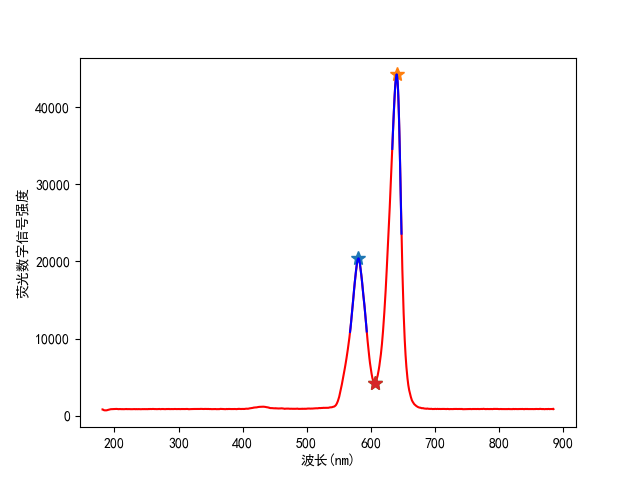
\includegraphics[scale=0.3]{黄红波峰特征值提取.png} \label{1}
    }
    \subfigure[蓝绿波峰数据散点图]{
    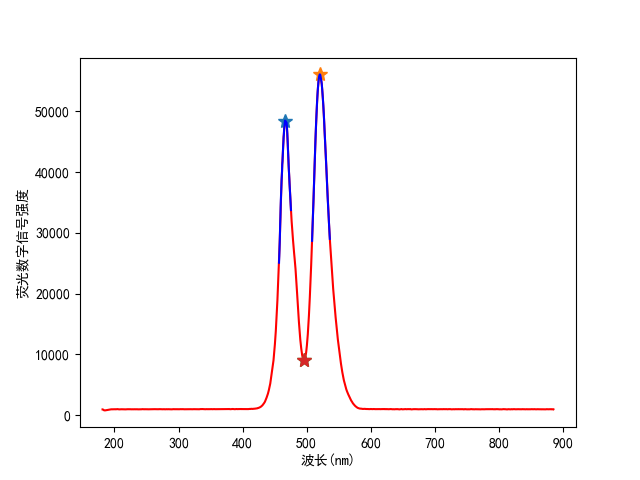
\includegraphics[scale=0.3]{蓝绿波峰特征值提取.png} \label{2} 
    }
    \subfigure[绿黄波峰数据散点图]{
    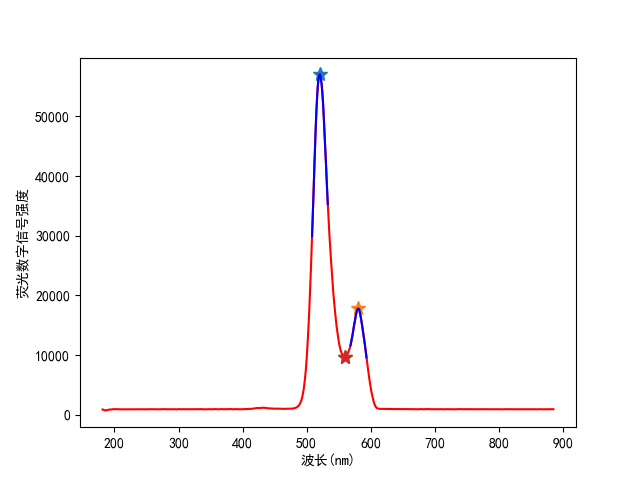
\includegraphics[scale=0.3]{绿黄波峰特征值提取.png}\label{3}
    }
    \quad
    \caption{附件1双峰光谱数据散点图}
\end{figure}

\subsubsection{预估半峰宽}
观测图1可知,波长小于400nm或大于700nm范围内三组数据的信号强度均较为平坦,相较于波峰的信号强度变化不大。故对第$i$组前100个数据的信号强度取平均数$y_{0i}$,表示峰底的信号强度。再将两个波峰的信号强度分别与峰底的信号强度取平均值,便可得到两个分峰的半峰高$y_{3i},y_{4i}$。继而检索信号强度高于半峰高的数据点,提取其对应波长的最小值与最大值,记为$x_{3i},x_{4i}$,则两峰的预测半峰宽$\Delta x_{1i},\Delta x_{2i}$可表示为:
\begin{equation}
\begin{cases}
\Delta x_{1i}=2(x_{1i}-x_{3i})\quad\mbox{对应横坐标范围}[x_{3i},x_{3i}+\Delta x_{1i}]\\
\Delta x_{2i}=2(x_{4i}-x_{2i})\quad\mbox{对应横坐标范围}[x_{4i}-\Delta x_{2i},x_{2i}]
\end{cases}
\end{equation}
位于半峰宽横坐标范围内的点在图1中用蓝色表示。



\subsubsection{预估数据整合}
初步估计得到的分峰波长、峰高及半峰宽如下表所示:
\begin{table}[!htbp]
    \centering
    \begin{tabular}{|c|c|c|c|}\hline
        参数名 &黄红&蓝绿&绿黄\\\hline
        第1个波峰的强度&20,393.84
        &48,481.82
        &57,039.24
        \\
        第2个波峰的强度&44,217.84
        &56,080.16
        &17,803.51
        \\
        第1个波谷的强度&4,287.12
        &9,010.17
        &9,644.65
        \\
        第1个峰的半峰宽(nm)&26.12
        &18.64
        &24.64
        \\
        第2个峰的半峰宽(nm)&14.66
        &31.50
        &25.30
        \\第1个波峰的中心波长(nm)&580.86
        &466.24
        &520.84
        \\第2个波峰的中心波长(nm)&640.77
        &520.49
        &580.86
        \\
        \hline
    \end{tabular}
    \caption{问题一分峰参数估计值}
    \label{问题一预估数据}
\end{table}
    

\subsection{模型建立}

\subsubsection{高斯函数拟合单峰光谱}
由假设一,理想状态下光谱宽度由荧光分子不规则运动导致的多普勒效应造成,设所有荧光分子在各自参考系中发出光的波长为$\lambda_{0}$ ,某时刻一荧光分子以速度$v$沿与观测者成$\theta$角方向做无规则运动,则根据多普勒效应,接收波长$\lambda$可表示为:
\begin{equation}
\lambda=\lambda_{0}\,(1-\frac{v}{c}\,cos\theta)\,{(1-\frac{v^2}{c^2})}^{-\frac{1}{2}} 
\end{equation}
荧光分子无规则运动的速度远低于光速,故可以忽略相对论效应,不妨设$v_1=v\,cos\theta$,则:
\begin{equation}
\lambda=\lambda_{0}\,(1-\frac{v}{c}\,cos\theta)=\lambda_{0}\,(1-\frac{v_1}{c})
\end{equation}
且荧光分子服从麦克斯韦速度分布律:
\begin{equation}
f\left(v_{1}\right) d v_{1}=\left(\frac{m}{2 \pi k{T}}\right)^{\frac{1}{2}} \cdot e^{-\frac{m {v_{1}}^2}{2kT}} d v_{1}
\end{equation}
记$\Delta\lambda=\lambda-\lambda_{0}$,则:
\begin{equation}
\frac{\Delta \lambda}{\lambda_{0}}=-\frac{v_{1}}{c}
\end{equation}
将式(5.2.4)代入(5.2.3):
\begin{equation}
f\left(\Delta\lambda\right) d \lambda=\left(\frac{m c^2}{2 \pi k{T} {\lambda_{0}}^2}\right)^{\frac{1}{2}} \cdot e^{-\frac{m {c}^2}{2kT}{\left(\frac{\Delta\lambda}{\lambda}\right)}^2} d \lambda
\end{equation}
整理可得:
\begin{equation}
f\left(\Delta\lambda\right) d \lambda=\frac{1}{\sqrt{2 \pi}} \left(\sqrt{ \frac{k{T} {\lambda_{0}}^2}{m c^2}}\right)^{-1} \cdot e^{-(\lambda-\lambda_{0})^2 \left(2 {\left(\sqrt{ \frac{k{T} {\lambda_{0}}^2}{m c^2}}\right)}^2\right)^{-1}}d \lambda
\end{equation}
发出$\lambda_{0}~\lambda_{0}+\Delta\lambda$波长光的荧光分子满足上述分布,而高斯函数形如:
\begin{equation}
f(x)=a e^{-\frac{(x-b)^{2}}{2 c^{2}}}\quad a=\frac{1}{\sigma \sqrt{2 \pi}}, b=\mu, c=\sigma    
\end{equation}
形式相同,故可用高斯函数拟合单峰光谱。

\subsubsection{最小二乘拟合复合光谱}
用高斯型函数模拟的单个谱峰形如:
$$
g(\lambda)=\frac{1}{\sqrt{2 \pi \sigma}} \mathrm{e}^{-\frac{(\lambda-\mu)^{2}}{2 \sigma^{2}}}=a\,e^{-\frac{(\lambda-\mu)^{2}}{2 \sigma^{2}}},
$$
其中$g(\lambda)$ 为关于光谱波长 $\lambda$ 的函数, $\mu, a$ 分别为谱线的中心波长和峰高,$\sigma$为半峰宽的$\frac{1}{2\sqrt{ln2} }$.\\
设区间 $[a, b]$ 内任一点以整数 $i$ $(i1,2, \cdots, N)$ 表示, 则以 $i$ 点为中心的高斯函数记作 :
$$
g_{i}(\lambda)=\frac{1}{\sqrt{2 \pi \sigma}} \mathrm{e}^{-\frac{(\lambda-i)^{2}}{2 \sigma_i^{2}}}=a_i\,e^{-\frac{(\lambda-i)^{2}}{2 \sigma_i^{2}}}
$$
则N峰叠加拟合谱图可表示为:
$$
f(\lambda) = \sum_{i=1}^{N} g_{i}(\lambda)=\sum_{i=1}^{N} a_i\,e^{-\frac{(\lambda-i)^{2}}{2 \sigma_i^{2}}}\quad (i=1,2, \cdots, N) 。
$$
设实际图谱为$f^{*}(\lambda)$,则$f(\lambda)$ 与 $f^{*}(\lambda)$ 的误差平方和函数定义为:
$$
E=\frac{1}{2} \sum\limits_{i=1}^{N}\left[f(\lambda)-f^{*}(\lambda)\right]^{2}
$$
寻找最小二乘法意义下的最优拟合函数 $f(\lambda)$, 实质上是确定函数 $E$ 的极小值问题。 

\subsection{模型求解}

\subsubsection{求解方法}
$E$ 是关于 $\left(a_{i}, \sigma_{i}\right)(i=1,2, \cdots, N)$ 的多元非线性函数, 用解析法直接求解极值存在困难,但可以通过数值迭代法进行。数值迭代法分为两类:一类是导数法,该方法以目标函数导数的负方向作为下一次迭代方向;另一类是直接法,该方法一般是在目标函数的导数难以得到的情况下,直接利用目标函数而不利用其导数来确定下一次迭代方向。一般而言,前者的计算效率比后者高\cite {最小二乘}。本文目标函数$E$的导数存在并较易得到,故采用导数法。
对 $E$ 关于 $a_{i}, \sigma_{i}(i=1,2, \cdots, N)$ 分别求偏导, 得到:
$$\begin{cases}
\frac{\partial E}{\partial a_{i}}=\sum\limits_{i=1}^{N}\left[f(\lambda )-f^{*}(\lambda )\right] \mathrm{e}^{-\frac{(\lambda -i)^{2}}{2 \sigma_{i}^{2}}} \\
\frac{\partial E}{\partial \sigma_{i}}=\sum\limits_{j=1}^{N}\left[f(\lambda)-f^{*}(\lambda)\right] \mathrm{e}^{-\frac{(j-i)^{2}}{2 \sigma_{i}^{2}}} \frac{a_{i}(\lambda-i)^{2}}{\sigma_{i}^{3}} 
\end{cases}$$
为了保证迭代收敛的稳定性, 引入惯性因子 $\alpha$ 后的调整公式如下:
$$\begin{cases}
\Delta a_{i}(t+1)=-p_{a} \frac{\partial E}{\partial a_{i}}+\alpha_{a} \Delta a_{i}(t), \\
\Delta \sigma_{i}(t+1)=-p_{\sigma} \frac{\partial E}{\partial \sigma_{i}}+\alpha_{\sigma} \Delta \sigma_{i}(t),
\end{cases}$$
$\Delta a_{i}(t)$ 和 $\Delta a_{i}(t+1)$ 分别为 $a_{i}$ 第 $t$ 次和 $t+1$ 次迭代调整量, $p_{a}$ 和 $\alpha_{a}$ 分别为其步长和惯性因子; $\Delta \sigma_{i}(t)$ 和 $\Delta \sigma_{i}(t+1)$ 分别为 $\sigma_{i}$ 第 $t$ 次和 $t+1$ 次迭代 调整量, $p_{\sigma}$ 和 $\alpha_{\sigma}$ 分别为其步长和惯性因子。\cite {最小二乘}
(算法实现详见附录A.2)
\subsubsection{结果及分析}
拟合得到的单峰与原始单峰线性相关系数如上表,线性相关系数均超过0.95,分峰效果较好

\begin{table}[h]
    \centering
    \begin{tabular}{|l|c|c|}\hline
        组别&\multicolumn{2}{c|}{线性相关系数}\\\hline
        黄红&0.996352008517681(黄)&0.959712648696846(红)\\
        蓝绿&0.981953296003524(蓝)&0.980693907202059(绿)\\
        绿黄&0.989571798229459(绿)&0.980693907202059(黄)\\
        \hline
    \end{tabular}
    \caption{问题一双峰分峰线性相关系数}
    \label{双峰分峰线性相关系数}
\end{table}

\begin{figure}[htbp]
    \centering
    \subfigure[黄红波峰数据散点图]{
    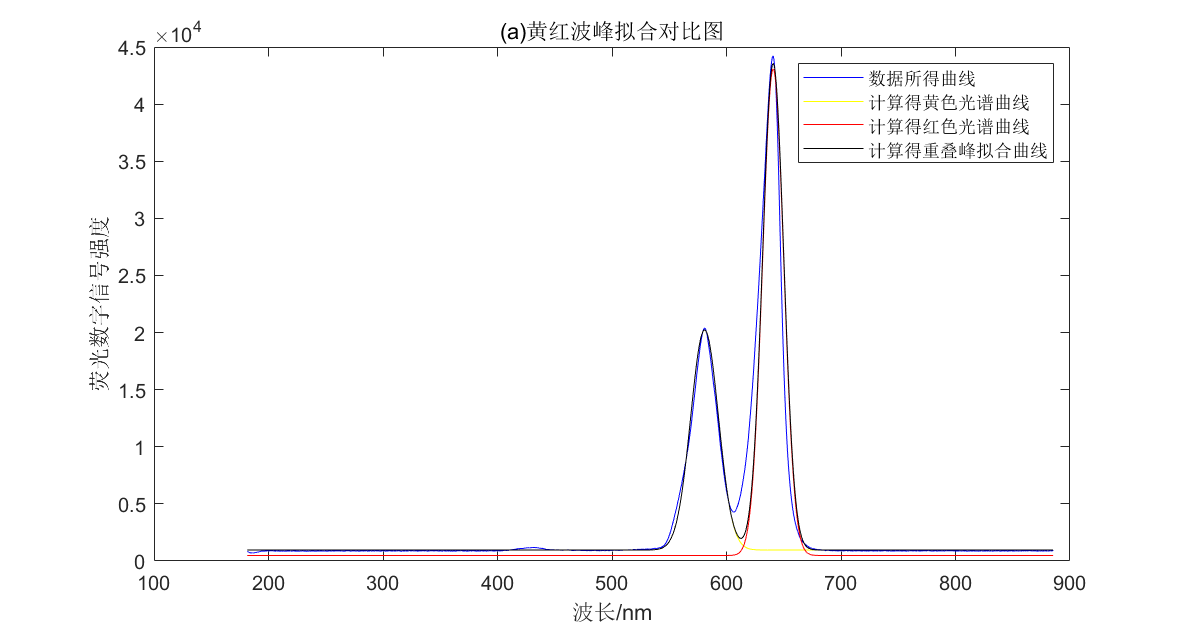
\includegraphics[scale=0.4]{黄红波峰拟合对比图.png} \label{1}
    }
    \subfigure[蓝绿波峰数据散点图]{
    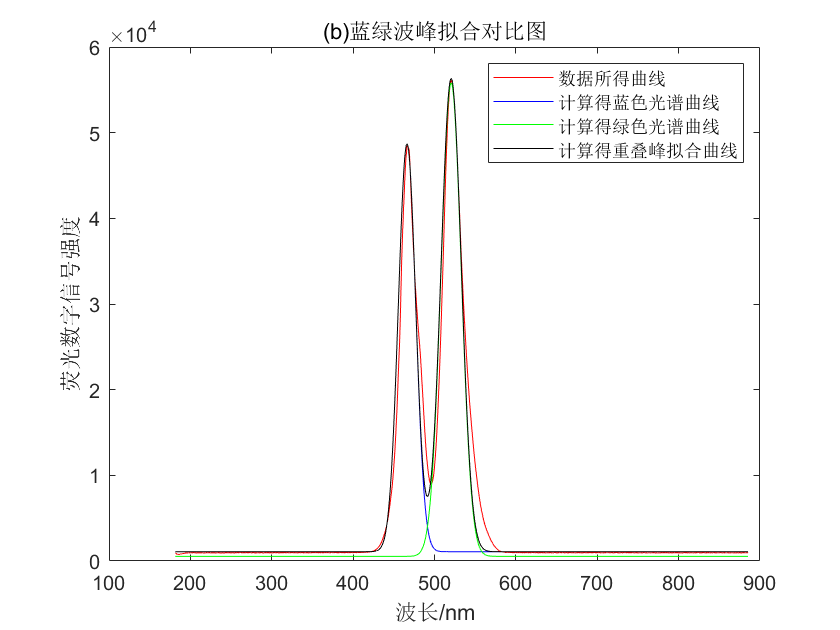
\includegraphics[scale=0.34]{蓝绿波峰拟合对比图.png} \label{2} 
    }
    \subfigure[绿黄波峰数据散点图]{
    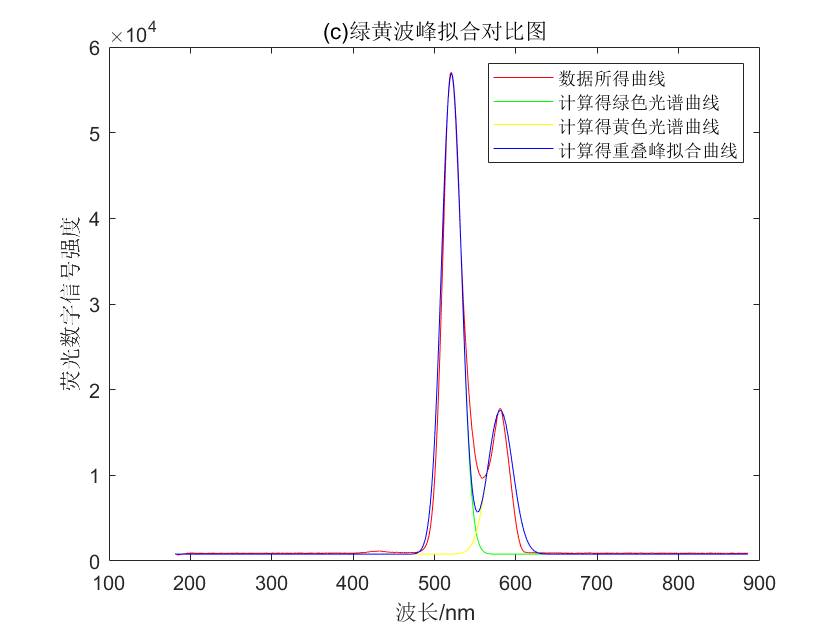
\includegraphics[scale=0.34]{绿黄波峰拟合对比图.png}\label{3}
    }
    \quad
    \caption{附件1双峰拟合对比图}
\end{figure}


{\centering\section{问题二模型的建立与求解}}

\subsection{数据处理}
\subsubsection{构建虚拟数据}
对给定的波长和半峰宽,在满足瑞利判据的前提下,令峰高比从1.000以0.333步长遍历至9.000,生成50组虚拟的单峰光谱数据,叠加得到25组双峰复合光谱数据。(程序与数据参见附录B.1)

\subsubsection{预估曲线参数}
预估双峰复合曲线的中心波长、峰高及半峰宽仍采用5.1的处理方法。绘制复合光谱数据散点图如图3,整合得到的预估数值见下表:
\begin{figure}[H]
    \centering
    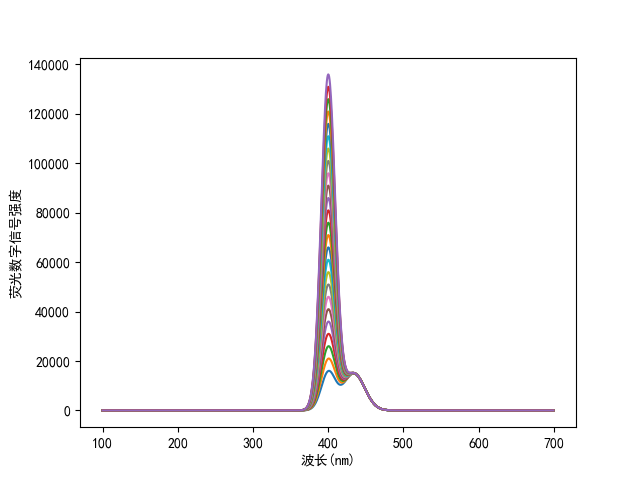
\includegraphics[scale=0.6]{峰高比1_to_9作图.png}
    \caption{问题二虚拟数据峰高比1-9散点图}
    \label{问题二虚拟数据峰高比1-9散点图}
\end{figure}
\newpage
注:半峰宽与中心波长单位为纳米(nm)
\begin{table}[h]
    \begin{tabular}{|c|c|c|c|c|c|c|}\hline
        峰高比&波峰1峰强&波峰2峰强&峰1半峰宽&峰2半峰宽&峰1中心波长&峰2中心波长\\\hline
        1.000&16,013.01
        &15,017.55
        &22.80
        &33.60
        &401.20
        &433.60\\

        1.333&20,991.78
        &15,025.32
        &21.60
        &33.60
        &400.60
        &433.60\\

        1.667&25,981.48
        &15,033.08
        &21.60
        &33.60
        &400.60
        &433.60\\

        2.000&30,971.18
        &15,040.85
        &22.80
        &33.60
        &400.60
        &433.60\\

        2.333&35,960.88
        &15,048.62
        &22.80
        &33.60
        &400.60
        &433.60\\

        2.667&40,950.58
        &15,056.39
        &22.80
        &33.60
        &400.60
        &433.60\\

        3.000&45,940.28
        &15,064.15
        &22.80
        &33.60
        &400.60
        &433.60\\

        3.333&50,937.50
        &15,071.92
        &21.60
        &33.60
        &400.00
        &433.60\\

        3.667&55,937.50
        &15,079.69
        &21.60
        &33.60
        &400.00
        &433.60\\

        4.000&60,937.50
        &15,087.46
        &21.60
        &33.60
        &400.00
        &433.60\\

        4.333&65,937.50
        &15,095.22
        &21.60
        &33.60
        &400.00
        &433.60\\

        4.667&70,937.50
        &15,102.99
        &21.60
        &33.60
        &400.00
        &433.60\\

        5.000&75,937.50
        &15,110.76
        &21.60
        &33.60
        &400.00
        &433.60\\

        5.333&80,937.50
        &15,120.32
        &21.60
        &34.80
        &400.00
        &433.00\\

        5.667&85,937.50
        &15,130.08
        &21.60
        &34.80
        &400.00
        &433.00\\

        6.000&90,937.50
        &15,139.85
        &21.60
        &34.80
        &400.00
        &433.00\\

        6.333&95,937.50
        &15,149.61
        &21.60
        &34.80
        &400.00
        &433.00\\

        6.667&100,937.50
        &15,159.38
        &21.60
        &34.80
        &400.00
        &433.00\\

        7.000&105,937.50
        &15,169.14
        &21.60
        &34.80
        &400.00
        &433.00\\

        7.333&110,937.50
        &15,178.91
        &21.60
        &34.80
        &400.00
        &433.00\\

        7.667&115,937.50
        &15,189.41
        &21.60
        &36.00
        &400.00
        &432.40\\

        8.000&120,937.50
        &15,201.63
        &21.60
        &36.00
        &400.00
        &432.40\\

        8.333&125,937.50
        &15,213.86
        &21.60
        &36.00
        &400.00
        &432.40\\

        8.667&130,937.50
        &15,226.09
        &21.60
        &36.00
        &400.00
        &432.40\\

        9.000&135,937.50
        &15,238.52
        &21.60
        &37.20
        &400.00
        &431.80\\

        
        \hline
    \end{tabular}
    \caption{问题二虚拟分峰参数估计值}
    \label{问题二虚拟分峰参数估计值}
\end{table}
\newpage

\subsection{模型建立与求解}
使用5.2,5.3中的最小二乘拟合模型,得出线性相关系数,相对误差如下表所示:
\begin{table}[h]
    \centering
    \begin{tabular}{|c|c|c|c|c|}\hline
        峰高比&复合峰相关系数&峰1相关系数&峰2相关系数&相对误差\\\hline
        1.000&0.999671354&	0.998875278&	0.999783442&0.000586865\\

        1.333&0.999561478&	0.998866441&	0.999573098&0.000785398\\

        1.667&0.999480277&	0.998874813&	0.999425651&0.000934852\\

        2.000&0.99942004&	0.998877857&	0.999252767&0.001048149\\

        2.333&0.999919491&	0.999969415&	0.999357757&0.000145843\\

        2.667&0.999935198&	0.999976571&	0.999357506&0.000117902\\

        3.000&0.999946464&	0.999983288&	0.999382956&9.79582E-05\\

        3.333&0.999955443&	0.999986436&	0.999382982&8.18016E-05\\

        3.667&0.999962401&	0.999988774&	0.999383011&6.92287E-05\\

        4.000&0.999967886&	0.999990556&	0.999383041&5.92804E-05\\

        4.333&0.999972276&	0.999991946&	0.999383071&5.12899E-05\\

        4.667&0.99997584&	0.999993051&	0.999383101&4.47848E-05\\

        5.000&0.999977549&	0.999994605&	0.999400705&4.18223E-05\\

        5.333&0.99998012&	0.999995374&	0.99940071&3.70869E-05\\

        5.667&0.999935222&	0.999979045&	0.997394604&0.000120417\\

        6.000&0.999941874&	0.999981103&	0.99737909&0.000108163\\

        6.333&0.999947599&	0.999983038&	0.99737913&9.76204E-05\\

        6.667&0.999952526&	0.99998469&	0.997379172&8.85338E-05\\

        7.000&0.99995653&	0.999985583&	0.997306931&8.1072E-05\\

        7.333&0.999960275&	0.999986867&	0.997306982&7.41515E-05\\

        7.667&0.999920726&	0.999974266&	0.993979483&0.000148172\\

        8.000&0.99992703&	0.999976369&	0.993980259&0.00013649\\

        8.333&0.999932615&	0.999978224&	0.993981035&0.000126129\\

        8.667&0.999889894&	0.999963688&	0.98833575&0.000205733\\

        9.000&0.999847926&	0.999951322&	0.981786848&0.000284283\\
        \hline
    \end{tabular}
    \caption{问题二拟合误差}
\end{table}

随着峰高比的增大,拟合的线性相关系数越低,相对误差越大,分峰效果越差。
\newpage


{\centering\section{问题三模型的建立与求解}}

\subsection{数据处理}

\subsubsection{三峰复合光谱分峰模型}
利用附件 2 中的两组数据分别绘制散点图,如图4所示。

光谱图象形状清晰曲线规则,推测噪声对光谱峰信号的干扰较小,仍使用\verb|signal.find_peaks|函数寻找峰强极值点的方法预测各分峰峰高及中心波长,筛选出波峰波谷处的极值点并在图上用星形标记(详见附录C.1代码)。用波峰处极值点的信号强度作为各分峰的预估峰强,检索波峰对应的荧光波长作为各分峰的预估中心波长,得到峰强与中心波长的粗略估计值。

\begin{figure}[htbp]
    \centering
    \subfigure[黄红波峰数据散点图]{
    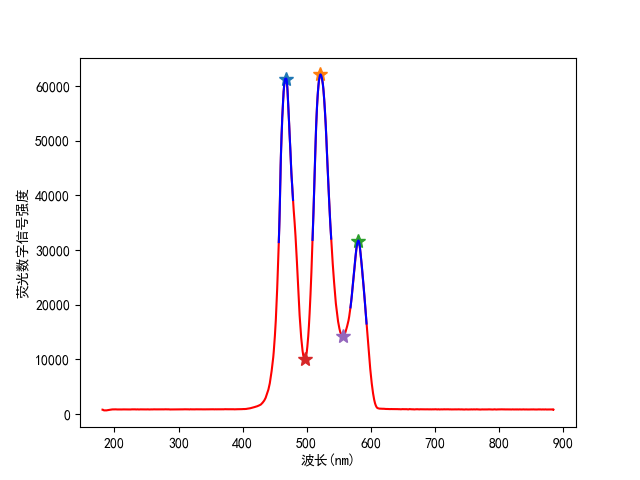
\includegraphics[scale=0.4]{蓝绿黄的波峰特征值提取.png} \label{1}
    }
    \subfigure[蓝绿波峰数据散点图]{
    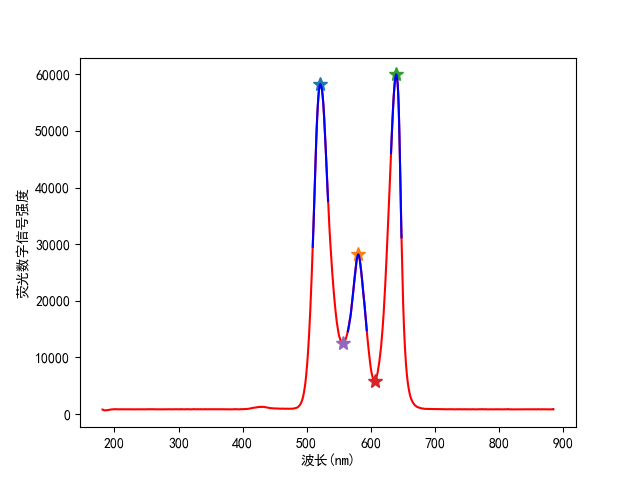
\includegraphics[scale=0.4]{绿黄红的波峰特征值提取.png} \label{2} 
    }
        \caption{附件2三峰光谱数据散点图}
\end{figure}
受到三峰复合光谱两个波谷的限制,中间波峰的半峰宽可能无法用5.1.2的方法估计得出。随着复合光谱峰数的增加,需要建立更普适的半峰宽估计方法。若多峰复合光谱由多个对称的单峰光谱叠加形成,且重叠度相对不高,则可使用以下流程方法预估半峰宽:
\begin{figure}[H]
    \centering
    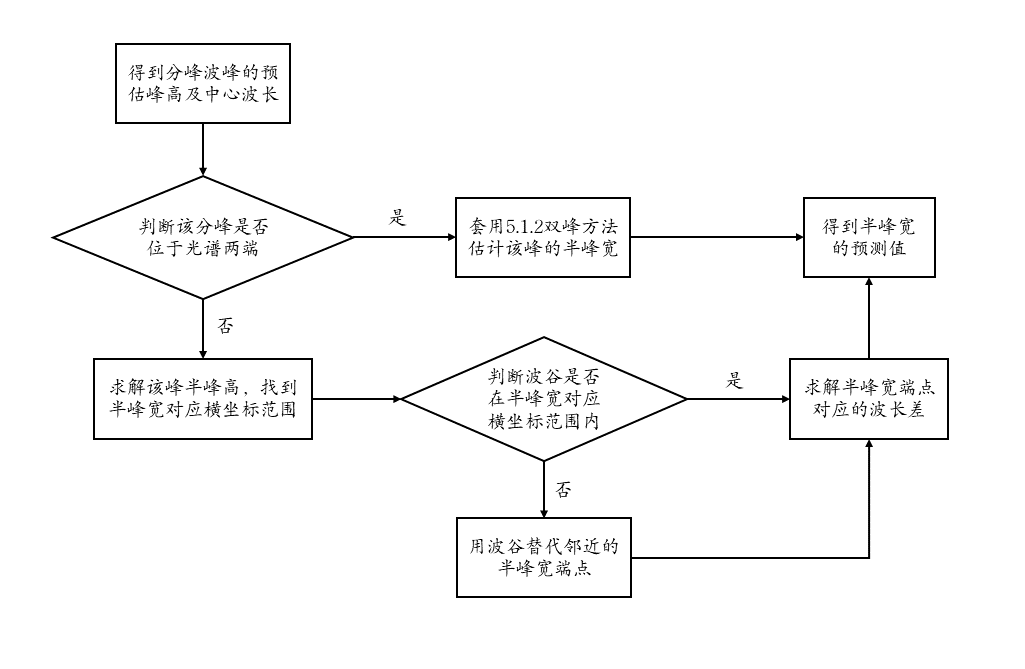
\includegraphics[scale=0.55]{半峰宽预估程序框图.PNG}
    \caption{多峰复合光谱预估分峰半峰宽流程图}
\end{figure}
图四的数据中,各波谷均位于分峰的预估半峰宽之外,只需求出半峰宽端点对应的波长即可对单峰的半峰宽做出估计。位于半峰宽横坐标范围内的点在图4中用蓝色表示,初步估计得到的分峰波长、峰高及半峰宽整合如下表所示:
\begin{table}[h]
    \centering
    \begin{tabular}{|c|c|c|}\hline
        参数名 &蓝绿黄&绿黄红\\\hline
        第1个波峰的强度&61,357.43
        &58,223.72
        \\        
        第2个波峰的强度&62,113.91
        &28,198.34
        \\
        第3个波峰的强度&31,745.64
        &59,963.55
        \\
        第1个波谷的强度&10,049.51
        &5,845.72
        \\
        第2个波谷的强度&14,315.76
        &12,475.11
        \\
        第1个峰的半峰宽(nm)&22.22
        &23.92
        \\
        第2个峰的半峰宽(nm)&24.62
        &32.32
        \\
        第3个峰的半峰宽(nm)&24.76
        &16.06
        \\第1个波峰的中心波长(nm)&467.67
        &521.54
        \\
        第2个波峰的中心波长(nm)&521.54
        &580.51
        \\
        第3个波峰的中心波长(nm)&580.86
        &639.76
        \\
        \hline
    \end{tabular}
    \caption{问题三三峰复合光谱分峰参数估计值}
    \label{tab:Margin_settings}
\end{table}

\subsubsection{四峰复合光谱分峰模型}
利用附件 2 中的两组数据分别绘制散点图,如图7所示。

\begin{figure}[htbp]
    \centering
    \subfigure[4-1波峰数据散点图]{
    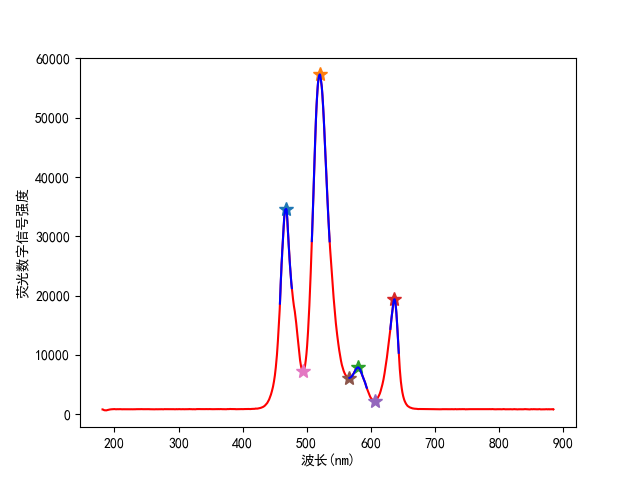
\includegraphics[scale=0.3]{4-1的波峰特征值提取.png} \label{1}
    }
    \subfigure[4-2波峰数据散点图]{
    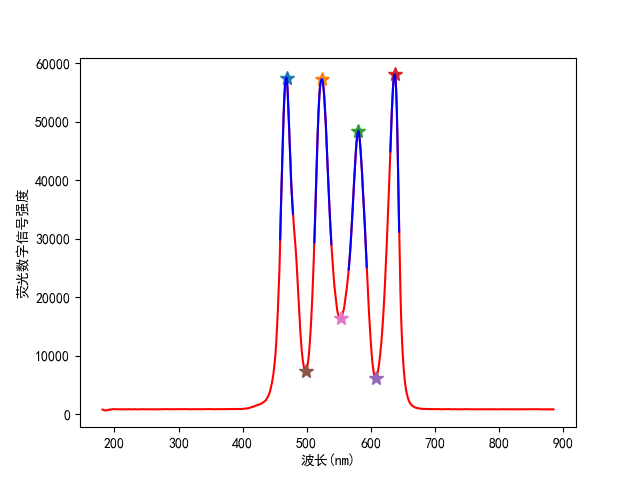
\includegraphics[scale=0.3]{4-2的波峰特征值提取.png} \label{2} 
    }
    \subfigure[4-3波峰数据散点图]{
    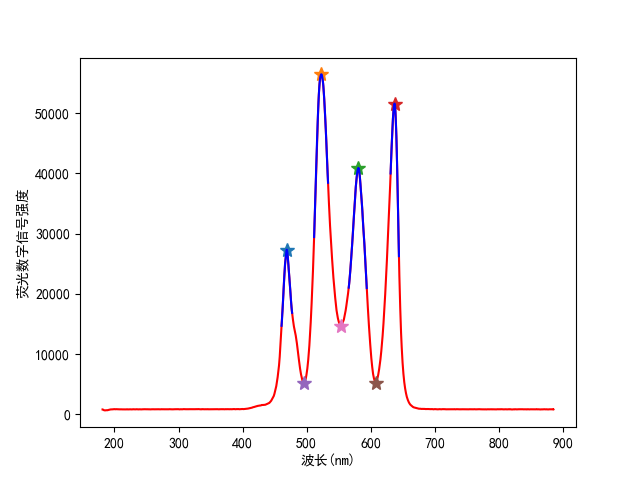
\includegraphics[scale=0.3]{4-3的波峰特征值提取.png}\label{3}
    }
    \subfigure[4-4波峰数据散点图]{
    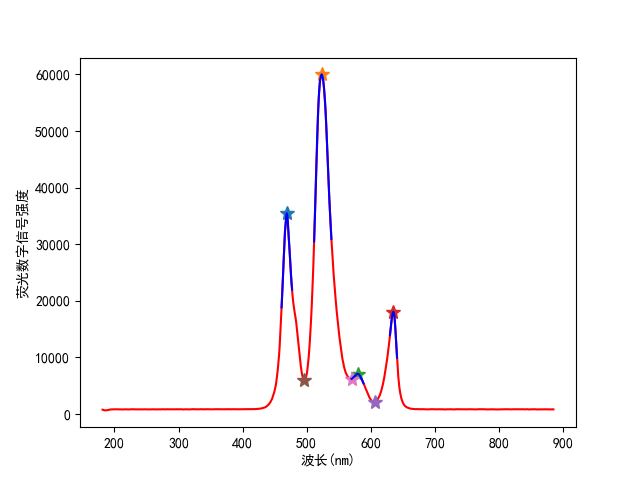
\includegraphics[scale=0.3]{4-4的波峰特征值提取.png} \label{1}
    }
    \subfigure[4-5波峰数据散点图]{
    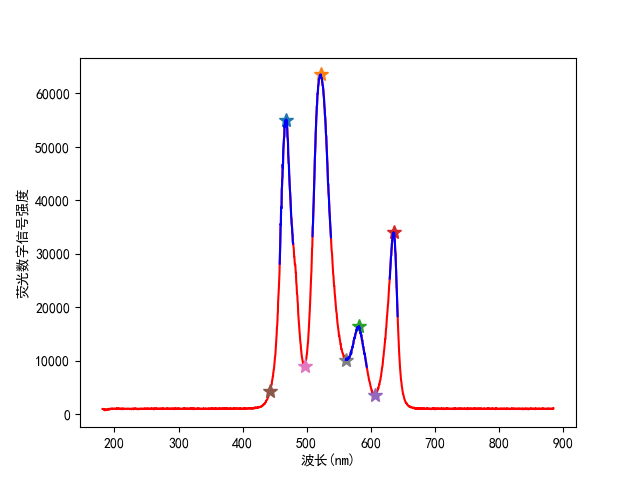
\includegraphics[scale=0.3]{4-5的波峰特征值提取.png} \label{1}
    }
    \quad
    \caption{附件2四峰光谱数据散点图}
\end{figure}
使用7.1.1中多峰复合光谱预估单峰参数的方法,用\verb|signal.find_peaks|函数筛选出波峰波谷处的极值点并在图上用星形标记(详见附录C.1代码),以波峰处极值点的信号强度作为各分峰的预估峰强,通过检索得到各单峰的预估中心波长,再按图5的方法估得四峰复合光谱各分峰的半峰宽。位于半峰宽横坐标范围内的点在图 6 中用蓝色表示,初步估计得到的分峰波长、峰高及半峰宽整合如下表所示:
\begin{figure}[H]
    \centering
    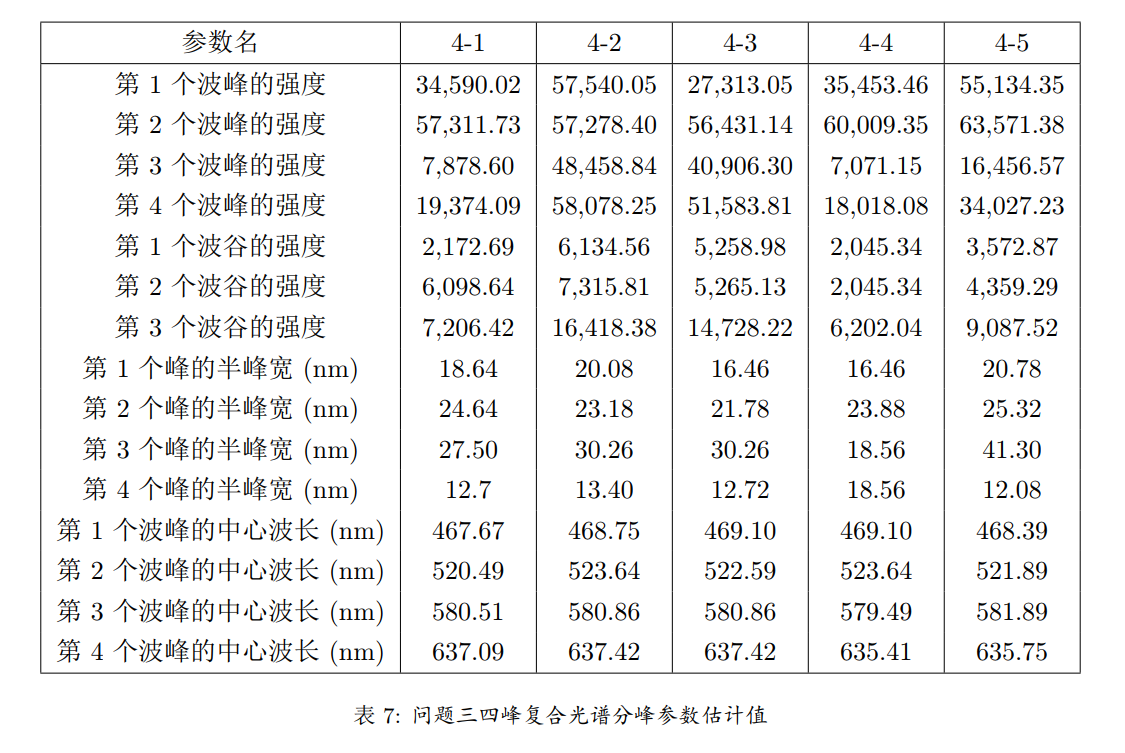
\includegraphics[scale=0.38]{四峰拆分预估参数.png}
    
\end{figure}

\newpage
\subsection{模型的建立与求解}
由5.2.2可知,有限个单峰光谱的复合均可用最小二乘拟合逼近,故仍使用最小二乘拟合模型,拟合图像及线性相关系数如下:
\subsubsection{三峰复合光谱分峰模型}

\begin{figure}[htbp]
    \centering
    \subfigure[黄红波峰数据散点图]{
    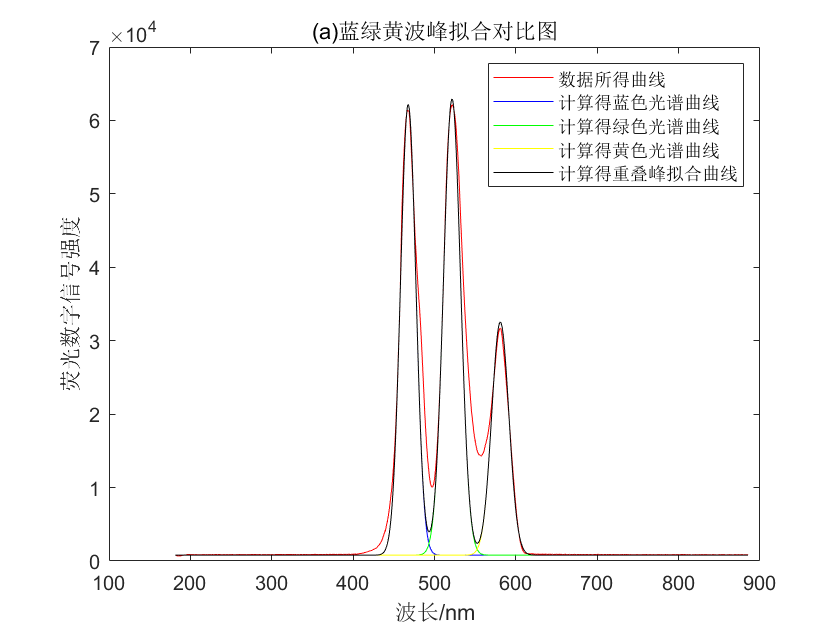
\includegraphics[scale=0.27]{蓝绿黄波峰拟合对比图.png} \label{1}
    }
    \subfigure[蓝绿波峰数据散点图]{
    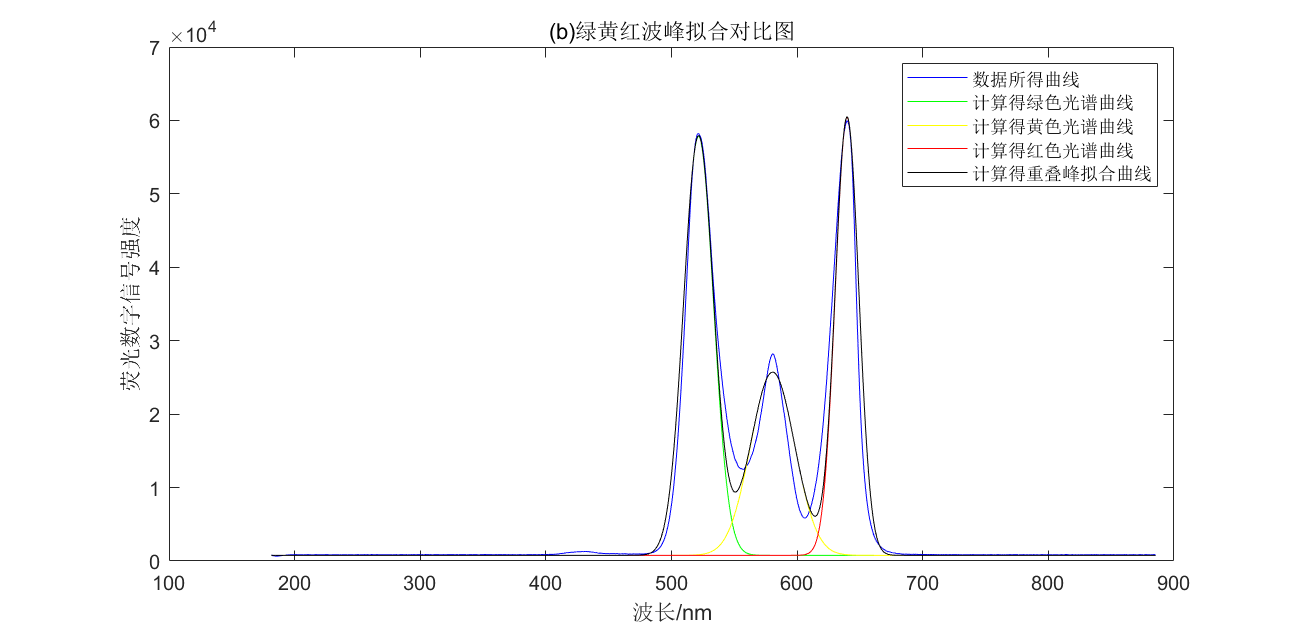
\includegraphics[scale=0.27]{绿黄红波峰拟合对比图.png} \label{2} 
    }
    
    \caption{附件2三峰拟合对比图}
\end{figure}

\begin{table}[h]
    \centering
    \begin{tabular}{|l|c|c|c|}\hline
        组别&\multicolumn{3}{c|}{线性相关系数}\\\hline
        蓝绿黄&0.991671208495265(蓝)&0.985592034458935(绿)&0.994994411962427(黄)\\
        绿黄红&0.985601173075390(绿)&0.960119254105144(黄)&0.977446030640229(红)\\
        \hline
    \end{tabular}
    \caption{问题三三峰分峰线性相关系数}
    \label{双峰分峰线性相关系数}
\end{table}
拟合得到的单峰与原始单峰线性相关系数如上表,线性相关系数均超过 0.96,分峰效果较好。

\subsubsection{四峰复合光谱分峰模型}

\begin{figure}[htbp]
    \centering
    \subfigure[4-1波峰数据散点图]{
    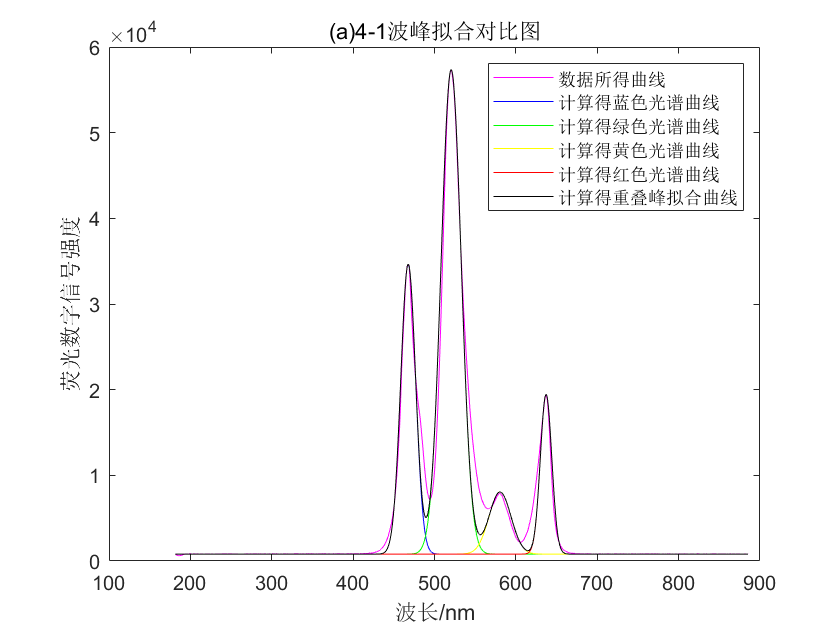
\includegraphics[scale=0.3]{4-1波峰拟合对比.png} \label{1}
    }
    \subfigure[4-2波峰数据散点图]{
    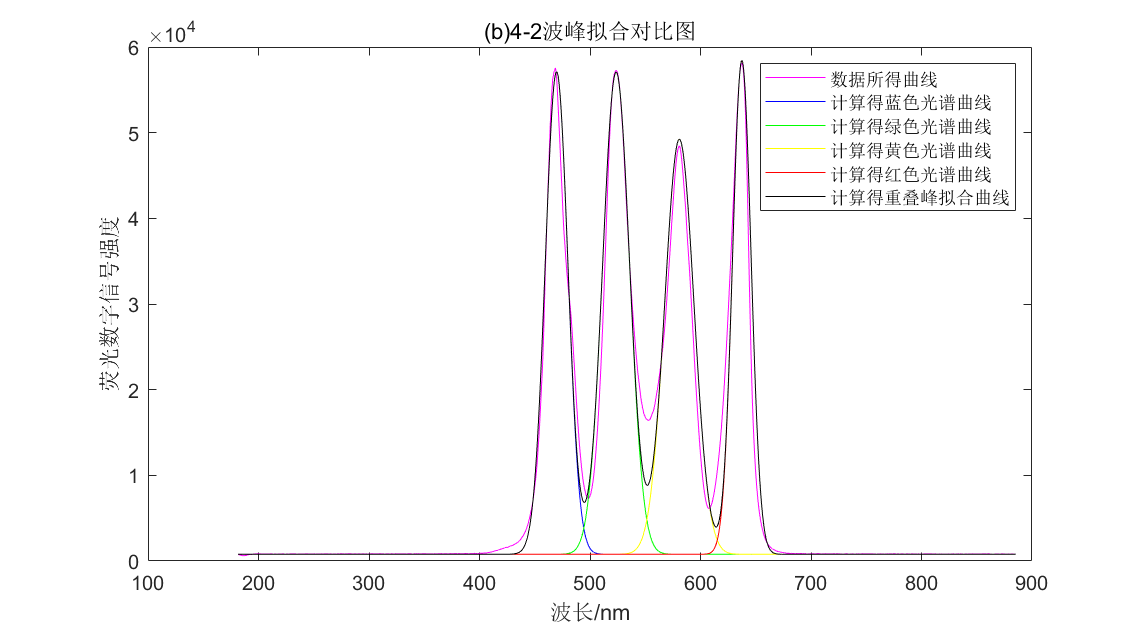
\includegraphics[scale=0.28]{4-2波峰拟合对比.png} \label{2} 
    }
    \subfigure[4-3波峰数据散点图]{
    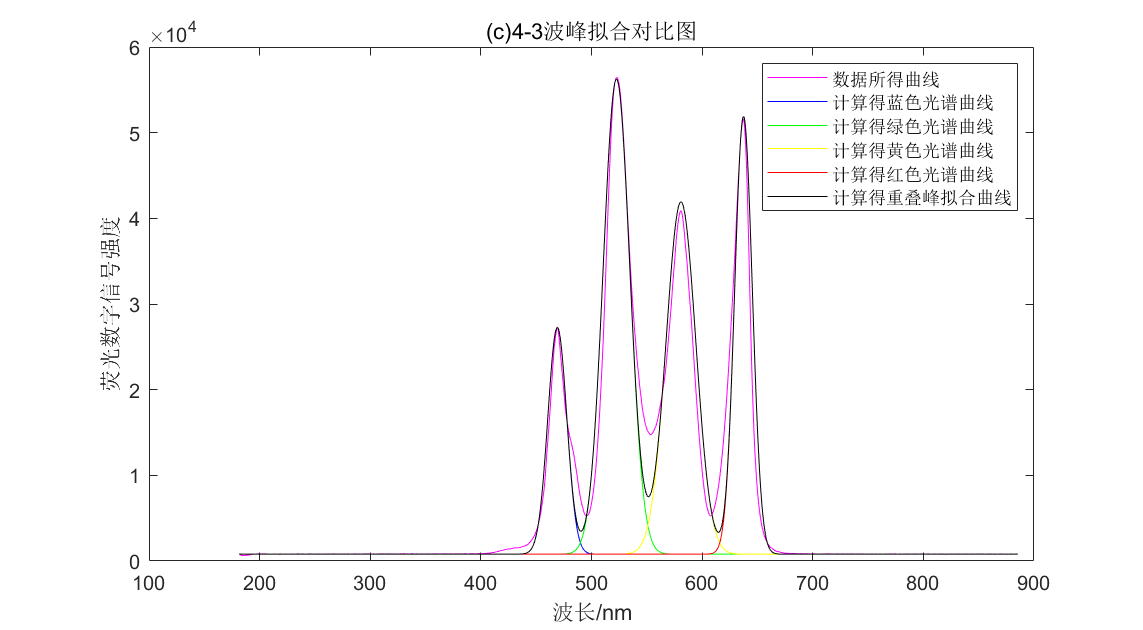
\includegraphics[scale=0.28]{4-3波峰拟合对比.png}\label{3}
    }
    \subfigure[4-4波峰数据散点图]{
    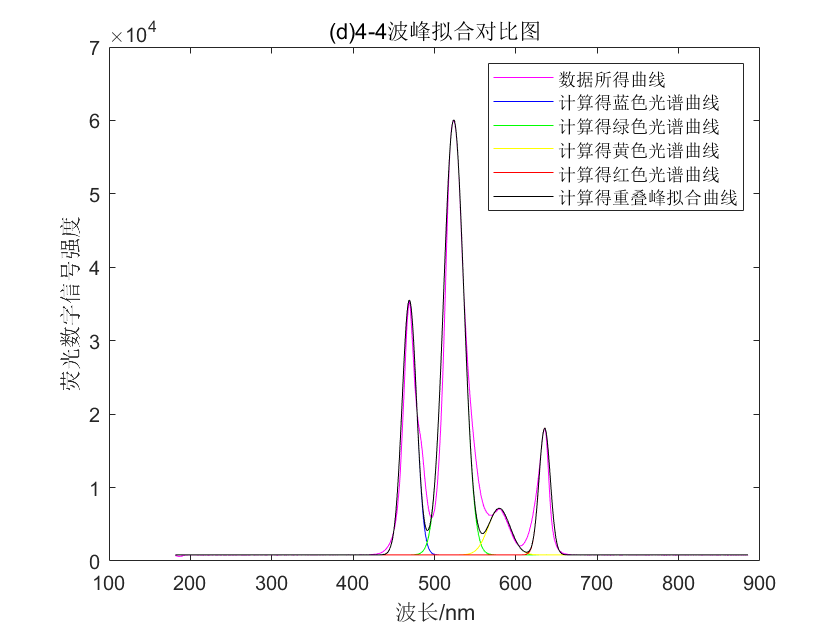
\includegraphics[scale=0.3]{4-4波峰拟合对比.png} \label{1}
    }
    \subfigure[4-5波峰数据散点图]{
    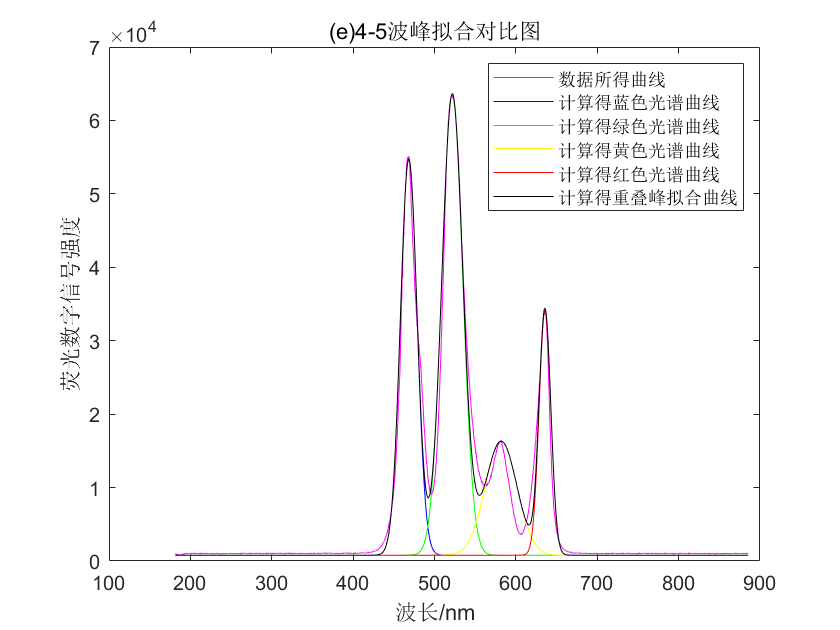
\includegraphics[scale=0.35]{4-5波峰拟合对比.png} \label{1}
    }
    \quad
    \caption{附件2四峰拟合对比图}
\end{figure}
\newpage

\begin{table}[h]
    \centering
    \begin{tabular}{|l|c|c|c|c|}\hline
        组别&\multicolumn{4}{c|}{线性相关系数}\\\hline
        4-1&0.981890272339212&0.988361262512770&0.993303698735636&0.946078922744599\\
        4-2&0.993051688216376&0.988145148099476&0.993585659587470&0.961451936899554\\
        4-3&   0.977870586000329

        &0.984178088708726
     
        &0.992467781010006
     
        &0.967302559133360
     \\
        4-4&0.979902760110044

        &0.988860682237004
     
       & 0.993567689721240
     
        &0.953985389100263\\
        4-5&0.990709862908278

        &0.989096003689477
     
        &0.935506690590112
     
        &0.971845763983573\\
        \hline
    \end{tabular}
    \caption{问题三三峰分峰线性相关系数}
    \label{双峰分峰线性相关系数}
\end{table}
拟合得到的单峰与原始单峰线性相关系数如上表,线性相关系数均超过 0.93,分峰效果尚可。



{\centering\section{问题四模型的建立与求解}}
\subsection{数据处理}


    
\subsection{模型建立与求解}
最小二乘拟合模型,得出拟合图像及线性相关系数如下(程序详见附件)
\begin{figure}[H]
    \centering
    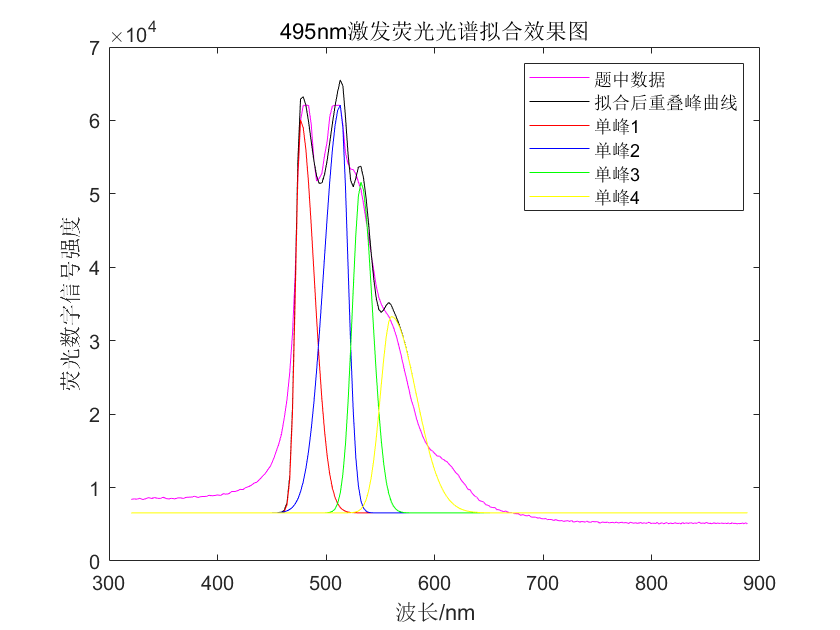
\includegraphics[scale=0.6]{非对称拟合.png}
    \caption{问题二虚拟数据峰高比1-9散点图}
    \label{问题二虚拟数据峰高比1-9散点图}
\end{figure}
线性相关系数为0.984060259416489,拟合程度较好

















{\centering\section{参考文献}}
\begingroup  % 去掉thebibliography环境自带的“参考文献”标题
\renewcommand{\section}[2]{}
\begin{thebibliography}{99}
    
\bibitem{最小二乘}
胡耀垓,张晓星,赵正予,冯 波. 光谱重叠峰的曲线拟合解析策略与实现[J] . 信息系统工程 . 2012.5 .第35卷第5期. 76-82

\end{thebibliography}
\endgroup







\newpage

{\centering\section*{附录}}
\appendix


\section{问题一相关数据及代码}
\subsection{数据处理python代码}
\begin{python}
    #中心波长and峰强and半波宽
from optparse import Values
from turtle import distance
from scipy.signal import argrelextrema
from numpy import *
from pandas import *
from matplotlib.pyplot import *
from scipy import signal
for filenames in ['黄红','蓝绿','绿黄']:
    a=read_excel(filenames+'.xlsx')
    print(filenames)
    b=a['波长(nm)']
    c=a['荧光数字信号强度']
    d=-c
    excelarray=[]
    #方法1
    num_peak_3=signal.find_peaks(c,distance=100)
    num_peak_4=signal.find_peaks(d,distance=100)
    peak=[]
    leastpeak=[]
    dictionary={}
    plot(b,c,'r',label='original values')
    #极大值
    for ii in range(len(num_peak_3[0])):
        if c[num_peak_3[0][ii]]>5000:          #剔除坏点
            plot(b[num_peak_3[0][ii]],c[num_peak_3[0][ii]],'*',markersize=10) 
            print('峰值的波长',b[num_peak_3[0][ii]],'nm');print('峰值的荧光数字信号强度',c[num_peak_3[0][ii]])
            peak.append(num_peak_3[0][ii])          #波峰的索引
            excelarray.append(['第{}个波峰的强度'.format(peak.index(num_peak_3[0][ii])+1),c[num_peak_3[0][ii]]])
            excelarray.append(['第{}个波峰的中心波长'.format(peak.index(num_peak_3[0][ii])+1),b[num_peak_3[0][ii]]])
    #极小值
    for ii in range(len(num_peak_4[0])):
        if d[num_peak_4[0][ii]]>-10000:          #剔除坏点
            dictionary[d[num_peak_4[0][ii]]]=num_peak_4[0][ii]          #用-极小值做键,索引做值
            leastpeak.append(d[num_peak_4[0][ii]])
    least_min=[min(leastpeak)]
    plot(b[dictionary[least_min[0]]],-least_min[0],'*',markersize=10) 
    for i in range(len(least_min)):
        plot(b[dictionary[least_min[i]]],-least_min[i],'*',markersize=10) 
        print('峰谷的波长',b[dictionary[least_min[i]]],'nm');print('峰谷的荧光数字信号强度',-least_min[i])
        excelarray.append(['第{}个波谷的强度'.format(i+1),-least_min[i]])
    c_base=c[0:100].mean()

    for i in 0,1:  
            height=c[peak[i]]-c_base

            xs=[x for x in range(len(c)) if (c[x]-c_base)>(height/2) ]
            min_b_distance=abs(min(b[x] for x in xs)-b[peak[i]]);max_b_distance=abs(max(b[x] for x in xs)-b[peak[i]])   
            if min_b_distance <= max_b_distance:                #取到正确的半波宽的对应横坐标(波长)x
                xs=[x for x in xs if abs(b[x]-b[peak[i]]) <= min_b_distance]
                bxs=[b[x] for x in xs]
                cxs=[c[x] for x in xs]
                # plot(min(b[xs]))
                plot(bxs,cxs,'b-')
                lambda_b=2*min_b_distance          #根据高斯函数对称性得到的半波宽
                print('第',i+1,'个峰的复合图像上的半峰宽为:',lambda_b,'nm')
            else:
                xs=[x for x in xs if abs(b[x]-b[peak[i]]) <= max_b_distance]
                bxs=[b[x] for x in xs]
                cxs=[c[x] for x in xs]
                plot(bxs,cxs,'b-')
                # plot(min(b[xs]),min(c[xs]),'x');plot(max(b[xs]),min(c[xs]),'x')
                lambda_b=2*max_b_distance
                print('第',i+1,'个峰的复合图像上的半峰宽为:',lambda_b,'nm')
            excelarray.append(['第{}个峰的半峰宽'.format(i+1),lambda_b])
    rcParams['font.sans-serif']=['SimHei']
    rcParams['axes.unicode_minus']=False
    xlabel('波长(nm)')
    ylabel('荧光数字信号强度')
    name=filenames+'波峰特征值提取.png'
    savefig(name)
    df=DataFrame(excelarray,columns=['index','values'])
    df.to_excel(filenames+'的特征值数据.xlsx')
    show()
\end{python}



\section{问题二相关数据及代码}
\subsection{数据处理python代码}
(1)创建单峰虚拟数据
\begin{python}
#单峰
from cmath import sqrt
import numpy as np 
import pandas as pd
import matplotlib.pyplot as plt
import openpyxl

def gauss(x,a,b,c):             #只有峰强和波长是变量
    y=a*np.exp(-(x-b)**2/(2*c**2))
    return y
c1=22/(2*sqrt(np.log(4)))
c2=34/(2*sqrt(np.log(4)))
x=np.arange(100,700,0.6)
b1=400;b2=434
a1=np.arange(15000,140000,5000)
a2=15000
arrayt=[]

for i in a1:
    y=[]
    arrayt=[[]]
    for j in x:
        y.append(gauss(j,i,b1,c1))        
    for t in range(len(x)):
        arrayt.append([x[t],float(y[t])])
    
    df=pd.DataFrame(arrayt,columns=['波长(nm)','荧光数字信号强度'])
    df.to_excel('峰高比{:.3f}的单峰1.xlsx'.format(i/a2),sheet_name='单峰1')
    plt.plot(x,y)


for i in a1:
    y=[]
    arrayt=[[]]
    for j in x:
        y.append(gauss(j,a2,b2,c2))        
    for t in range(len(x)):
        arrayt.append([x[t],float(y[t])])
    
    df=pd.DataFrame(arrayt,columns=['波长(nm)','荧光数字信号强度'])
    df.to_excel('峰高比{:.3f}的单峰2.xlsx'.format(i/a2),sheet_name='单峰2')
    plt.plot(x,y)
    
\end{python}
(2)创建重叠峰峰数据
\begin{python}
from cmath import sqrt
import numpy as np 
import pandas as pd
import matplotlib.pyplot as plt
import openpyxl

def gauss(x,a,b,c):             #只有峰强和波长是变量
    y=a*np.exp(-(x-b)**2/(2*c**2))
    return y
c1=22/(2*sqrt(np.log(4)))
c2=34/(2*sqrt(np.log(4)))
x=np.arange(100,700,0.6)
b1=400;b2=434
a1=np.arange(15000,140000,5000)
a2=15000
arrayt=[]

for i in a1:
    y=[]
    arrayt=[[]]
    for j in x:
        y.append(gauss(j,i,b1,c1)+gauss(j,a2,b2,c2))        
    for t in range(len(x)):
        arrayt.append([x[t],float(y[t])])
    
    df=pd.DataFrame(arrayt,columns=['波长(nm)','荧光数字信号强度'])
    df.to_excel('峰高比{:.3f}.xlsx'.format(i/a2),sheet_name='复合光谱')
    plt.plot(x,y)
plt.rcParams['font.sans-serif']=['SimHei']
plt.xlabel('波长(nm)')
plt.ylabel('荧光数字信号强度')
plt.savefig('峰高比1_to_9作图.png')
plt.show()   
\end{python}
(3)预估中心波长,峰高及半峰宽
\begin{python}
from turtle import distance
from scipy.signal import argrelextrema
from numpy import *
from pandas import *
from matplotlib.pyplot import *
from scipy import signal
for filenames in ['峰高比1.000.xlsx','峰高比1.333.xlsx','峰高比1.667.xlsx','峰高比2.000.xlsx','峰高比2.333.xlsx','峰高比2.667.xlsx','峰高比3.000.xlsx','峰高比3.333.xlsx','峰高比3.667.xlsx','峰高比4.000.xlsx','峰高比4.333.xlsx','峰高比4.667.xlsx','峰高比5.000.xlsx','峰高比5.333.xlsx','峰高比5.667.xlsx','峰高比6.000.xlsx','峰高比6.333.xlsx','峰高比6.667.xlsx','峰高比7.000.xlsx','峰高比7.333.xlsx','峰高比7.667.xlsx','峰高比8.000.xlsx','峰高比8.333.xlsx','峰高比8.667.xlsx','峰高比9.000.xlsx']:
    a=read_excel(filenames)
    print(filenames)
    b=a['波长(nm)']
    c=a['荧光数字信号强度']
    d=-c
    excelarray=[]
    #方法5
    num_peak_3=signal.find_peaks(c,distance=50)
    num_peak_4=signal.find_peaks(d,distance=50)
    peak=[]
    leastpeak=[]
    dictionary={}
    # plot(b,c,'r',label='original values')
    #极大值
    for ii in range(len(num_peak_3[0])):
        if c[num_peak_3[0][ii]]>5000:          #剔除坏点
            # plot(b[num_peak_3[0][ii]],c[num_peak_3[0][ii]],'*',markersize=10) 
            print('峰值的波长',b[num_peak_3[0][ii]],'nm');print('峰值的荧光数字信号强度',c[num_peak_3[0][ii]])
            peak.append(num_peak_3[0][ii])          #波峰的索引
            excelarray.append(['第{}个波峰的强度'.format(peak.index(num_peak_3[0][ii])+1),c[num_peak_3[0][ii]]])
            excelarray.append(['第{}个波峰的中心波长'.format(peak.index(num_peak_3[0][ii])+1),b[num_peak_3[0][ii]]])
    #极小值
    for ii in range(len(num_peak_4[0])):
        if d[num_peak_4[0][ii]]>-20000:          #剔除坏点
            dictionary[d[num_peak_4[0][ii]]]=num_peak_4[0][ii]          #用-极小值做键,索引做值
            leastpeak.append(d[num_peak_4[0][ii]])
    least_min=[min(leastpeak)]
    # plot(b[dictionary[least_min]],-least_min,'*',markersize=10) 
    for i in range(len(least_min)):
        plot(b[dictionary[least_min[i]]],-least_min[i],'*',markersize=10) 
        print('峰谷的波长',b[dictionary[least_min[i]]],'nm');print('峰谷的荧光数字信号强度',-least_min[i])
        excelarray.append(['第{}个波谷的强度'.format(i+1),-least_min[i]])
    c_base=c[0:100].mean()

    for i in 0,1:  
        height=c[peak[i]]-c_base

        xs=[x for x in range(len(c)) if (c[x]-c_base)>(height/2) ]
        min_b_distance=abs(min(b[x] for x in xs)-b[peak[i]]);max_b_distance=abs(max(b[x] for x in xs)-b[peak[i]])   
        if min_b_distance <= max_b_distance:                #取到正确的半波宽的对应横坐标(波长)x
            xs=[x for x in xs if abs(b[x]-b[peak[i]]) <= min_b_distance]
            bxs=[b[x] for x in xs]
            cxs=[c[x] for x in xs]
            plot(bxs,cxs,'g-')
            lambda_b=2*min_b_distance
            print('第',i+1,'个峰的复合图像上的半波宽为:',lambda_b,'nm')
        else:
            xs=[x for x in xs if abs(b[x]-b[peak[i]]) <= max_b_distance]
            bxs=[b[x] for x in xs]
            cxs=[c[x] for x in xs]
            plot(bxs,cxs,'b-')
            lambda_b=2*max_b_distance
            print('第',i+1,'个峰的复合图像上的半波宽为:',lambda_b,'nm')
        excelarray.append(['第{}个峰的半峰宽'.format(i+1),lambda_b])
    df=DataFrame(excelarray,columns=['index','values'])
    df.to_excel(filenames+'的特征值数据.xlsx')
    
\end{python}



\section{问题三相关数据及代码}
\subsection{数据处理python代码}
(1)三峰复合光谱分峰
\begin{python}
from fileinput import filename
from turtle import distance
from unicodedata import name
from scipy.signal import argrelextrema
from numpy import *
from pandas import *
from matplotlib.pyplot import *
from scipy import signal
import heapq
for filenames in ['蓝绿黄','绿黄红']:
    a=read_excel(filenames+'.xlsx')
    print(filenames)
    b=a['波长(nm)']

    c=a['荧光数字信号强度']
    d=-c
    #方法
    num_peak_3=signal.find_peaks(c,distance=50)
    num_peak_4=signal.find_peaks(d,distance=20)
    peak=[]
    leastpeak=[]
    excelarray=[]
    dictionary={}
    plot(b,c,'r',label='original values')
    #极大值
    for ii in range(len(num_peak_3[0])):
        if c[num_peak_3[0][ii]]>20000:          #剔除坏点
            plot(b[num_peak_3[0][ii]],c[num_peak_3[0][ii]],'*',markersize=10) 
            print('峰值的波长',b[num_peak_3[0][ii]],'nm');print('峰值的荧光数字信号强度',c[num_peak_3[0][ii]])
            peak.append(num_peak_3[0][ii])          #波峰的索引
            excelarray.append(['第{}个波峰的强度'.format(peak.index(num_peak_3[0][ii])+1),c[num_peak_3[0][ii]]])
            excelarray.append(['第{}个波峰的中心波长'.format(peak.index(num_peak_3[0][ii])+1),b[num_peak_3[0][ii]]])
    #极小值
    for ii in range(len(num_peak_4[0])):
        if  d[num_peak_4[0][ii]]<-5000 :          #剔除坏点
            dictionary[d[num_peak_4[0][ii]]]=num_peak_4[0][ii]          #用-极小值做键,索引做值
            leastpeak.append(d[num_peak_4[0][ii]])
    least_min=heapq.nlargest(2,leastpeak)
    for i in range(len(least_min)):
        plot(b[dictionary[least_min[i]]],-least_min[i],'*',markersize=10) 
        print('峰谷的波长',b[dictionary[least_min[i]]],'nm');print('峰谷的荧光数字信号强度',-least_min[i])
        excelarray.append(['第{}个波谷的强度'.format(i+1),-least_min[i]])
    c_base=c[1:100].mean()
    for i in range(len(peak)):  
        height=c[peak[i]]-c_base

        xs=[x for x in range(len(c)) if (c[x]-c_base)>(height/2) ]
        min_b_distance=min(abs(min(b[x] for x in xs)-b[peak[i]]),abs(b[peak[i]]-b[dictionary[least_min[0]]]),abs(b[peak[i]]-b[dictionary[least_min[1]]]))
        max_b_distance=min(abs(max(b[x] for x in xs)-b[peak[i]]),abs(b[peak[i]]-b[dictionary[least_min[0]]]),abs(b[peak[i]]-b[dictionary[least_min[1]]]))   
        if min_b_distance <= max_b_distance:                #取到正确的半波宽的对应横坐标(波长)x
            xs=[x for x in xs if abs(b[x]-b[peak[i]]) <= min_b_distance]
            bxs=[b[x] for x in xs]
            cxs=[c[x] for x in xs]
            plot(bxs,cxs,'b-')
            t=min(min_b_distance,abs(min(bxs)-b[peak[i]]))
            lambda_b=2*t
            print('第',i+1,'个峰的复合图像上的半波宽为:',lambda_b,'nm')
        else:
            xs=[x for x in xs if abs(b[x]-b[peak[i]]) <= max_b_distance]
            bxs=[b[x] for x in xs]
            cxs=[c[x] for x in xs]
            plot(bxs,cxs,'b-')
            t=min(max_b_distance,abs(min(bxs)-b[peak[i]]))
            lambda_b=2*t
            print('第',i+1,'个峰的复合图像上的半波宽为:',lambda_b,'nm')
        excelarray.append(['第{}个峰的半峰宽'.format(i+1),lambda_b])
    rcParams['font.sans-serif']=['SimHei']
    rcParams['axes.unicode_minus']=False

    xlabel('波长(nm)')
    ylabel('荧光数字信号强度')
    name=filenames + '的波峰特征值提取.png'
    savefig(name)

    df=DataFrame(excelarray,columns=['index','values'])
    df.to_excel(filenames+'的特征值数据.xlsx')
    show()    
\end{python}
(2)四峰复合光谱分峰
\begin{python}
from turtle import distance
from scipy.signal import argrelextrema
from numpy import *
from pandas import *
from matplotlib.pyplot import *
from scipy import signal
import heapq
for filenames in ['4-1','4-2','4-3','4-4']:
    a=read_excel(filenames+'.xlsx')
    print(filenames)
    b=a['波长(nm)']
    c=a['荧光数字信号强度']
    d=-c
    excelarray=[]
    #方法1
    num_peak_3=signal.find_peaks(c,distance=50)
    num_peak_4=signal.find_peaks(d,distance=20)
    peak=[]
    leastpeak=[]
    dictionary={}
    plot(b,c,'r',label='original values')
    #极大值
    for ii in range(len(num_peak_3[0])):
        if c[num_peak_3[0][ii]]>6000:          #剔除坏点
            plot(b[num_peak_3[0][ii]],c[num_peak_3[0][ii]],'*',markersize=10) 
            print('峰值的波长',b[num_peak_3[0][ii]],'nm');print('峰值的荧光数字信号强度',c[num_peak_3[0][ii]])
            peak.append(num_peak_3[0][ii])          #波峰的索引
            excelarray.append(['第{}个波峰的强度'.format(peak.index(num_peak_3[0][ii])+1),c[num_peak_3[0][ii]]])
            excelarray.append(['第{}个波峰的中心波长'.format(peak.index(num_peak_3[0][ii])+1),b[num_peak_3[0][ii]]])
    #极小值
    for ii in range(len(num_peak_4[0])):
        if  d[num_peak_4[0][ii]]<-2000 :          #剔除坏点
            dictionary[d[num_peak_4[0][ii]]]=num_peak_4[0][ii]          #用-极小值做键,索引做值
            leastpeak.append(d[num_peak_4[0][ii]])
    least_min=heapq.nlargest(3,leastpeak)
    for i in range(len(least_min)):
        plot(b[dictionary[least_min[i]]],-least_min[i],'*',markersize=10) 
        print('峰谷的波长',b[dictionary[least_min[i]]],'nm');print('峰谷的荧光数字信号强度',-least_min[i])
        excelarray.append(['第{}个波谷的强度'.format(i+1),-least_min[i]])
    c_base=c[1:100].mean()
    for i in range(len(peak)):  
        height=c[peak[i]]-c_base

        xs=[x for x in range(len(c)) if (c[x]-c_base)>(height/2) ]
        min_b_distance=min(abs(min(b[x] for x in xs)-b[peak[i]]),abs(b[peak[i]]-b[dictionary[least_min[0]]]),abs(b[peak[i]]-b[dictionary[least_min[1]]]),abs(b[peak[i]]-b[dictionary[least_min[2]]]))
        max_b_distance=min(abs(max(b[x] for x in xs)-b[peak[i]]),abs(b[peak[i]]-b[dictionary[least_min[0]]]),abs(b[peak[i]]-b[dictionary[least_min[1]]]),abs(b[peak[i]]-b[dictionary[least_min[2]]]))   
        if min_b_distance <= max_b_distance:                #取到正确的半波宽的对应横坐标(波长)x
            xs=[x for x in xs if abs(b[x]-b[peak[i]]) <= min_b_distance]
            bxs=[b[x] for x in xs]
            cxs=[c[x] for x in xs]
            plot(bxs,cxs,'b-')
            t=min(min_b_distance,abs(min(bxs)-b[peak[i]]))
            lambda_b=2*t
            print('第',i+1,'个峰的复合图像上的半波宽为:',lambda_b,'nm')
        else:
            xs=[x for x in xs if abs(b[x]-b[peak[i]]) <= max_b_distance]
            bxs=[b[x] for x in xs]
            cxs=[c[x] for x in xs]
            plot(bxs,cxs,'b-')
            t=min(max_b_distance,abs(min(bxs)-b[peak[i]]))
            lambda_b=2*t
            print('第',i+1,'个峰的复合图像上的半波宽为:',lambda_b,'nm')
        excelarray.append(['第{}个峰的半峰宽'.format(i+1),lambda_b])
    rcParams['font.sans-serif']=['SimHei']
    xlabel('波长(nm)')
    ylabel('荧光数字信号强度')
    name=filenames + '的波峰特征值提取.png'
    savefig(name)
    df=DataFrame(excelarray,columns=['index','values'])
    df.to_excel(filenames+'的特征值数据.xlsx')
    show()        
a=read_excel('4-5.xlsx')
print('4-5.xlsx')
b=a['波长(nm)']
c=a['荧光数字信号强度']
d=-c
#取得特征值
num_peak_3=signal.find_peaks(c,distance=100)
num_peak_4=signal.find_peaks(d,distance=50)
peak=[]
leastpeak=[]
excelarray=[]
dictionary={}
plot(b,c,'r',label='original values')
#极大值
for ii in range(len(num_peak_3[0])):
    if c[num_peak_3[0][ii]]>6000:          #剔除坏点
        plot(b[num_peak_3[0][ii]],c[num_peak_3[0][ii]],'*',markersize=10) 
        print('峰值的波长',b[num_peak_3[0][ii]],'nm');print('峰值的荧光数字信号强度',c[num_peak_3[0][ii]])
        peak.append(num_peak_3[0][ii])          #波峰的索引
        excelarray.append(['第{}个波峰的强度'.format(peak.index(num_peak_3[0][ii])+1),c[num_peak_3[0][ii]]])
        excelarray.append(['第{}个波峰的中心波长'.format(peak.index(num_peak_3[0][ii])+1),b[num_peak_3[0][ii]]])
#极小值
for ii in range(len(num_peak_4[0])):
    if  d[num_peak_4[0][ii]]<-2000 and b[num_peak_4[0][ii]]>min(b[peak]):          #剔除坏点
        dictionary[d[num_peak_4[0][ii]]]=num_peak_4[0][ii]          #用-极小值做键,索引做值
        leastpeak.append(d[num_peak_4[0][ii]])
least_min=heapq.nlargest(3,leastpeak)
for i in range(len(least_min)):
        plot(b[dictionary[least_min[i]]],-least_min[i],'*',markersize=10) 
        print('峰谷的波长',b[dictionary[least_min[i]]],'nm');print('峰谷的荧光数字信号强度',-least_min[i])
        excelarray.append(['第{}个波谷的强度'.format(i+1),-least_min[i]])
c_base=c[1:100].mean()
for i in range(len(peak)):  
    height=c[peak[i]]-c_base

    xs=[x for x in range(len(c)) if (c[x]-c_base)>(height/2) ]
    min_b_distance=min(abs(min(b[x] for x in xs)-b[peak[i]]),abs(b[peak[i]]-b[dictionary[least_min[0]]]),abs(b[peak[i]]-b[dictionary[least_min[1]]]),abs(b[peak[i]]-b[dictionary[least_min[2]]]))
    max_b_distance=min(abs(max(b[x] for x in xs)-b[peak[i]]),abs(b[peak[i]]-b[dictionary[least_min[0]]]),abs(b[peak[i]]-b[dictionary[least_min[1]]]),abs(b[peak[i]]-b[dictionary[least_min[2]]]))   
    if min_b_distance <= max_b_distance:                #取到正确的半波宽的对应横坐标(波长)x
        xs=[x for x in xs if abs(b[x]-b[peak[i]]) <= min_b_distance]
        bxs=[b[x] for x in xs]
        cxs=[c[x] for x in xs]
        plot(bxs,cxs,'b-')
        t=min(min_b_distance,abs(min(bxs)-b[peak[i]]))
        lambda_b=2*t
        print('第',i+1,'个峰的复合图像上的半波宽为:',lambda_b,'nm')
    else:
        xs=[x for x in xs if abs(b[x]-b[peak[i]]) <= max_b_distance]
        bxs=[b[x] for x in xs]
        cxs=[c[x] for x in xs]
        plot(bxs,cxs,'b-')
        t=min(max_b_distance,abs(min(bxs)-b[peak[i]]))
        lambda_b=2*t
        print('第',i+1,'个峰的复合图像上的半波宽为:',lambda_b,'nm')
    excelarray.append(['第{}个峰的半峰宽'.format(i+1),lambda_b])
rcParams['font.sans-serif']=['SimHei']
xlabel('波长(nm)')
ylabel('荧光数字信号强度')
savefig('4-5的波峰特征值提取.png')
df=DataFrame(excelarray,columns=['index','values'])
df.to_excel('4-5的特征值数据.xlsx')
show()
    
\end{python}





\section{问题四相关数据及代码}
\subsection{数据处理python代码}
\begin{python}
from turtle import distance
from scipy.signal import argrelextrema
from numpy import *
from pandas import *
from matplotlib.pyplot import *
from scipy import signal
import heapq

a=read_excel('partial_twice.xlsx')
b=a['波长']
c=a['二次处理后的峰强']
d=-c
#方法1
num_peak_3=signal.find_peaks(c,distance=5)
num_peak_4=signal.find_peaks(d,distance=5)
peak=[]
leastpeak=[]
dictionary={}
excelarray=[]
new_peaklist=[]
plot(b,c,'r',label='original values')
#极大值
for ii in range(len(num_peak_3[0])):
    if c[num_peak_3[0][ii]]>40:          #剔除坏点
        new_peaklist.append(num_peak_3[0][ii])
        plot(b[num_peak_3[0][ii]],c[num_peak_3[0][ii]],'*',markersize=10) 
        print('峰值{}的波长'.format(new_peaklist.index(num_peak_3[0][ii])+1),b[num_peak_3[0][ii]],'nm');print('峰值的荧光数字信号强度',c[num_peak_3[0][ii]])
        peak.append(num_peak_3[0][ii])          #波峰的索引
        excelarray.append(['第{}个波峰的强度'.format(peak.index(num_peak_3[0][ii])+1),c[num_peak_3[0][ii]]])
        excelarray.append(['第{}个波峰的中心波长'.format(peak.index(num_peak_3[0][ii])+1),b[num_peak_3[0][ii]]])
#极小值
for ii in range(len(num_peak_4[0])):
    if  d[num_peak_4[0][ii]]>-50 and b[num_peak_4[0][ii]]>min(b[peak]):          #剔除坏点
        dictionary[d[num_peak_4[0][ii]]]=num_peak_4[0][ii]          #用-极小值做键,索引做值
        leastpeak.append(d[num_peak_4[0][ii]])
least_min=heapq.nlargest(5,leastpeak)               #取到三个波谷
for i in range(len(least_min)):
    
        plot(b[dictionary[least_min[i]]],-least_min[i],'*',markersize=10) 
        print('第{}个峰谷的波长'.format(i+1),b[dictionary[least_min[i]]],'nm');print('峰谷的荧光数字信号强度',-least_min[i])
        excelarray.append(['第{}个波谷的强度'.format(i+1),-least_min[i]])
        excelarray.append(['第{}个波谷的中心波长'.format(i+1),b[dictionary[least_min[i]]]])
xlabel('波长')
ylabel('二次微分处理后的信号强度')
title('复合光谱信号强度函数的二阶微分')
rcParams['font.sans-serif']=['SimHei']
rcParams['axes.unicode_minus']=False
df=DataFrame(excelarray,columns=['index','values'])
df.to_excel('partial_twice'+'的极大值极小值数据.xlsx')
show()   
\end{python}



\section{也可以插入matlab代码}
\begin{lstlisting}
    %论文1-熵权值求权重
    A=[58 38 14 8 57 10
    50 45 11 9 52 12
    42 47 8 12 50 15
    45 42 12 15 46 16
    47 44 13 10 49 13];%统计数据A 5x6
    [m,n]=size(A);
    h =max(A);%每一列最大值
    H=repmat(h,m,1);%向量h排列mx1的矩阵
    Mij=A./H%隶属度矩阵
    
    
    A2=sum(Mij);%Mij矩阵每一列求和
    A22=repmat(A2,m,1);%向量A2排列mx1的矩阵
    Qij=Mij./A22%隶属度矩阵每一列标准化
    
    
    Fj=-1/log(5)*Qij.*log(Qij);
    fj=sum(Fj);%熵值
    dj=1-fj;%差异系数
    v=dj/sum(dj)%权重系数
    B=Qij*v';%最终评价
    disp(B)%显示结果
    
\end{lstlisting}


\end{document}